\subsection{Complementary filter}
The complementary filter is used to combine the measurement data from the accelerometer and gyros in the two IMUs mounted on the Cubli frame. 
Based on the data from \appref{IMUMeasurementsAppendix} it can be seen that the accelerometer can detect changes in the angle, but has problems with measuring fast changes in the angle.\fxnote{source?, also reason for error seems to be fast and large?} 
The problem with the data from the gyro is an accumulating error which is caused by the integration done to convert angular velocity into an usable angle. It is also known that the gyros will exhibit a drifting error when experiencing small and slow movement.\fxnote{source on gyro error?, B}
 
As described in \secref{sec:Sensors} there are mounted two IMU's on the frame of the Cubli. One of the requirements are to have the Cubli balance in an upright position independently of the orientation of the baseplate.

Based on ... \fxnote{why did we choose an complementary filter?}

The two angle measurements of the IMU are sent through a filter and then summed in order to get an angle of the Cubli frame.
%Data from the accelerometer is used to calculate an angle of the Cubli frame.
%The gyroscope measurement is integrated to get the angle of the Cubli frame. Both measurements are done to find the change on the axis of movement of the Cubli.
 
This is done to counteract drift of the gyroscope and error of the accelerometer.\fxnote{elaborate on the errors} 

\begin{figure}[H]
	\begin{tikzpicture}[ auto,
thick,                         %<--setting line style
node distance=2cm,             %<--setting default node distance
scale=1.5,                     %<--|these two scale the whole thing
every node/.style={scale=1.5}, %<  |(always change both)
>=triangle 45 ]                %<--sets the arrowtype
\draw%--------------------------------------------------------------------------------------------

node[shape=coordinate][](acc) at (0,0){acc}			% start of acc signal path

node(lowpas) at (6,0) [block] {\Large $\ \frac{1}{\tau \cdot s + 1}$ }

node[shape=coordinate][](gyro) at (0,-2){}		% start of gyro signal path

node(integrate) at (3,-2) [block] {\Large $\frac{1}{s}$}

node(highpas) at (6,-2) [block] {\Large $\ \frac{\tau \cdot s}{\tau \cdot s + 1}$ }

node(sum) at (8,-1) [sum] {$\sum$}


node[shape=coordinate][](angle) at (10,-1){}		% output of the complementary filter
;

\draw[->](acc) -- node {accel$\_\theta_{F}$} (lowpas);
\draw[->](gyro) -- node {gyro$\_\omega_{F}$} (integrate);
\draw[->](integrate) -- node {} (highpas);

\draw[->](highpas) -| node {} (sum);
\draw[->](lowpas) -| node {} (sum);


\draw[->](sum) -- node {$\theta_{F}$} (angle);

\end{tikzpicture}

	\centering
	\caption{Block diagram of the complementary filter}
	\label{blockDrawingComplementaryFilter}
\end{figure}

%\begin{figure}[H] 
%	\centering
%	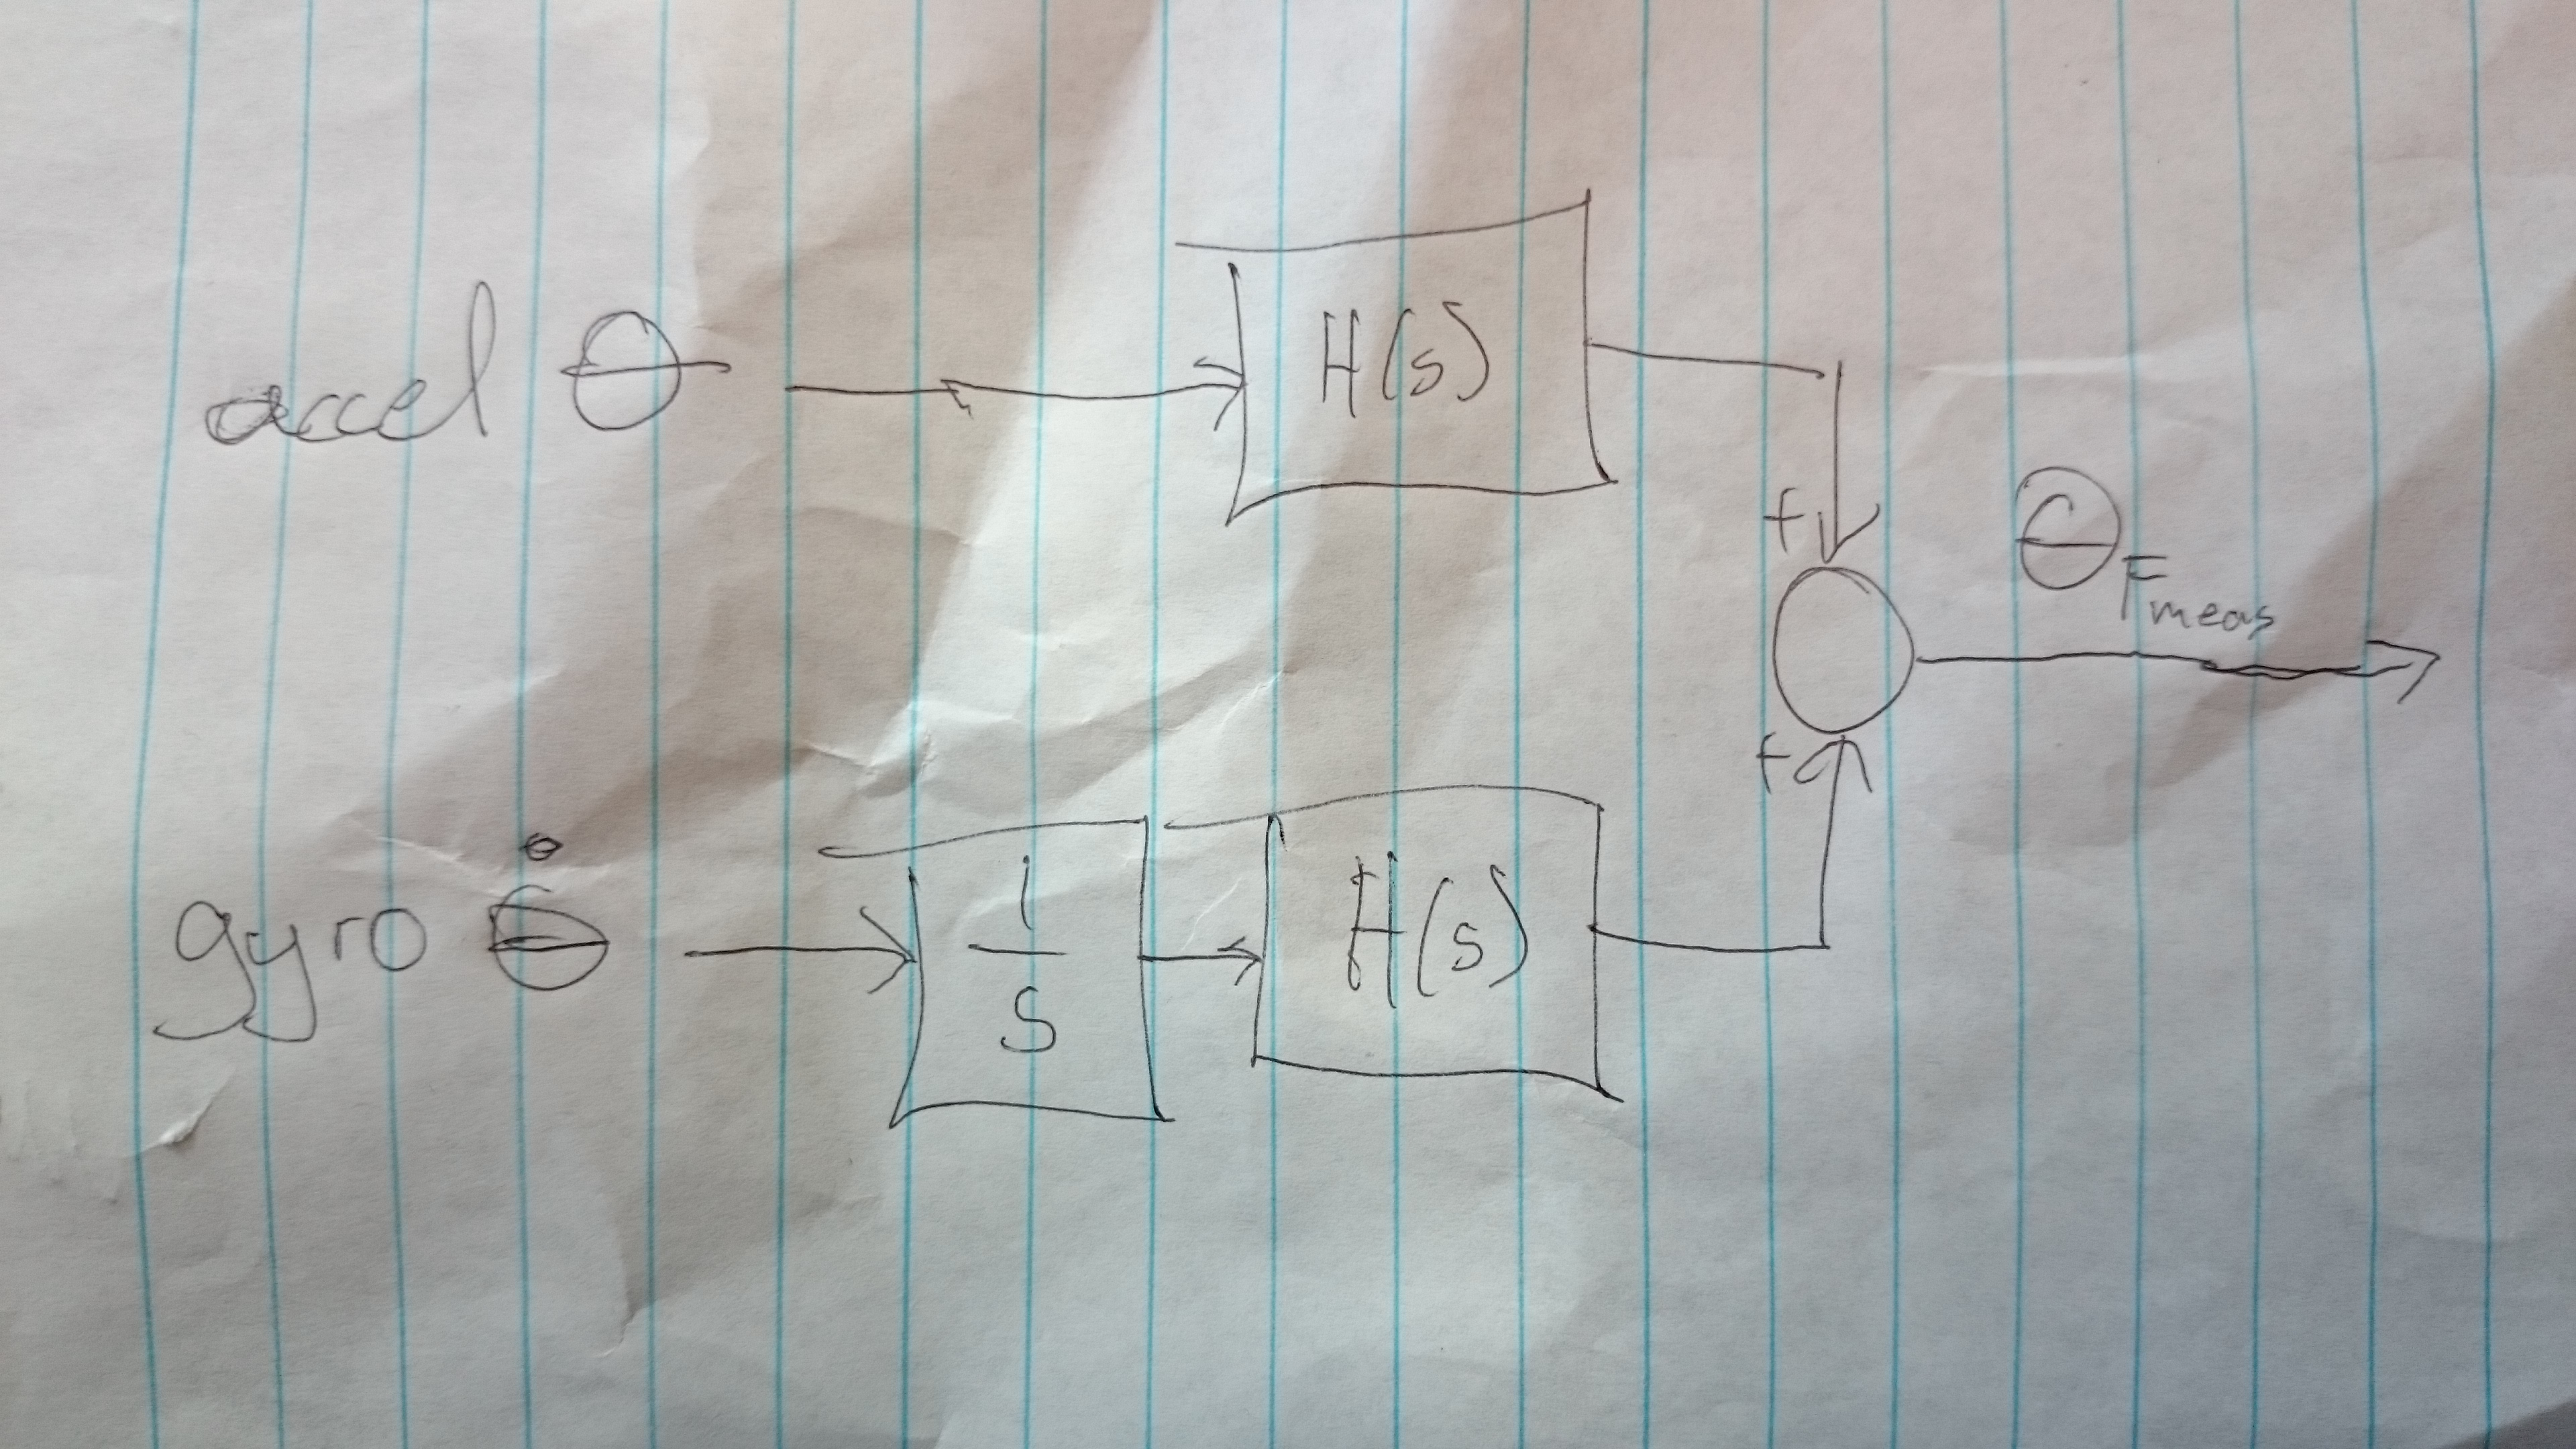
\includegraphics[scale=0.08]{figures/tempComplementaryFilter}
%	\caption{Sketch of the structure of the complementary filter. Measurements from the accelerometer are calculated into an angle on the axis of movement. Data from gyro is used to find the angular velocity on the axis of movement}
%	\label{blockComplementaryFilter}
%\end{figure}
%\fxnote{Make a proper sketch of the complementary filter, B}